
%%%%%%%%%%%%%%%%%%%% file icsc2024_template.tex %%%%%%%%%%%%%%%%%%%%%
% based on icsc2017 / 2022 template updated by Alex Hofmann for icsc2024 -- Nov. 2023
%
% This is the LaTeX source for the instructions to authors using
% the LaTeX document class 'llncs.cls' for contributions to
% the Lecture Notes in Computer Sciences series.
% http://www.springer.com/lncs       Springer Heidelberg 2006/05/04
%
% It may be used as a template for your own input - copy it
% to a new file with a new name and use it as the basis
% for your article.
%
% NB: the document class 'llncs' has its own and detailed documentation, see
% ftp://ftp.springer.de/data/pubftp/pub/tex/latex/llncs/latex2e/llncsdoc.pdf
%
%%%%%%%%%%%%%%%%%%%%%%%%%%%%%%%%%%%%%%%%%%%%%%%%%%%%%%%%%%%%%%%%%%%


\documentclass[runningheads,a4paper]{llncs}

\usepackage{amssymb}
\setcounter{tocdepth}{3}
\usepackage{graphicx}
% \usepackage{url}
\usepackage{hyperref}
\usepackage[margin=1.1in]{geometry}
\hypersetup{hidelinks}
\newcommand{\keywords}[1]{\par\addvspace\baselineskip
\noindent\keywordname\enspace\ignorespaces#1}

\pagestyle{headings}

\begin{document}

\mainmatter  % start of an individual contribution

% first the title is needed
\title{cloud-5:\\An Environment for Generating and Publishing Cloud Music}

% a short form should be given in case it is too long for the running head
\titlerunning{Running Title}


% TO GARANTEE THE DOUBLE BLIND REVIEW PROCESS, PLEASE
% KEEP THESE GENERIC AUTHOR NAMES AND INSTITUTIONS

\author{AuthorA\inst{1}\and AuthorB\inst{2} \thanks{I thank Dan Derks for introducing me to Tidal Cycles and Felix Roos for answering Strudel questions.}}
%
% if the names of the authors are too long for the running head, please use the format: AuthorA et al.
\authorrunning{AuthorA and AuthorB (or AuthorA et al. if too long)}

% the affiliations are given next; don't give your e-mail address
% unless you accept that it will be published
\institute{InstituteA \and InstituteB\\ \email{your.email@yourdomain.com}}

%
% NB: a more complex sample for affiliations and the mapping to the
% corresponding authors can be found in the file "llncs.dem"
% (search for the string "\mainmatter" where a contribution starts).
% "llncs.dem" accompanies the document class "llncs.cls".
%


\maketitle

% Should be 150 to 350 words.
\begin{abstract}
The advent of the World Wide Web, the standardization of HTML with adequate support for computer graphics and audio, and the introduction 
of WebAssembly have combined to create an environment suited to the \emph{online} production, publication, and presentation of art music, visual music, and 
related media at a professional standard of technical quality. A piece of music on the World Wide Web no longer need be merely 
a link to a downloadable soundfile or video, or even to an audio or visual stream. A piece can, indeed, be its own ``app" that is live code running in the listener's Web browser. I call this kind of music \emph{cloud music} because it exists only in the ``cloud,'' the omnipresent computing infrastructure of the Internet. I argue that this offers an entirely new environment for music that may, in the future, develop its own social context and function as an alternative means of disseminating art music in addition to live performances, discs, streams, and downloads. Here, I present and demonstrate \emph{cloud-5}, a collection of 
libraries and templates for producing cloud music including, among other things, fixed medium music, music that plays indefinitely, visuals that generate music, music that generates visuals, interactive music, and live coding. cloud-5 includes a WebAssembly build of the sound programming language and software synthesis system Csound, a WebAssembly build of the CsoundAC library for algorithmic composition including chords, scales, and voice-leading, the live coding application Strudel, and supporting code for menus, event handlers, GLSL shaders, and more. A cloud-5 piece thus exists as an HTML file that embeds Csound code and/or GLSL code and/or score generation code and/or Strudel code, in the context of a static Web site that can be served either locally (for composing and performing) or remotely on the World Wide Web (for publication).
\keywords{html5, webassembly, csound, algorithmic composition, visual music, live coding}
\end{abstract}

\section{Introduction}

This is a \LaTeX{} template to be used, together with the included Springer
class file \texttt{llncs.cls}, for the preparation of manuscripts for the
\textit{7\textsuperscript{th} International Csound Conference
\textemdash{} ICSC2024}.

The maximum paper length is four pages including abstract, figures, tables
and eventual references. An additional fifth page is accepted provided it
\textit{only} includes references.

To guarantee the double blind review process, manuscripts should not include
the author names nor affiliations. Please keep the generic names included in the
template.

\section{Paper Preparation}

When using \LaTeX\ together with the provided document class file, the text
is typeset automatically in Computer Modern Roman (CM) fonts. Please do
\emph{not} change the preset fonts or their size, or modify the class file
in any way.

Italic type may be used to emphasize words in running text. Bold type and
underlining should be avoided.

We recommend using the commands \verb+\label+ and \verb+\ref+ for
cross-references, the commands \verb+\bibitem+ and \verb+\cite+ for
references to the bibliography, and the command \verb+\url+ for URL
hyperlinks.


\subsection{Headings}

Only two levels of structure should be used throughout the document,
corresponding to the \verb+\section+ and \verb+\subsection+ sectioning
commands.

Headings should be capitalized, i.e., nouns, verbs, and all other words
except articles, prepositions, and conjunctions should be set with an
initial capital. Words joined by a hyphen are subject to a special rule: if
the first word can stand alone, the second word should be capitalized.

Here are some examples of headings: ``Developing a User-Friendly
Interface'', ``Processing Multi-track Audio Files with Granular Techniques''.

\subsection{Figures}

For integrating figures into the source file we recommend using the
standard \LaTeX{} \verb+graphics+ or \verb+graphicx+ package. These provide
the \verb+\includegraphics+ command. Please center the figures by using the
\verb+\centering+ declaration. Fig.~\ref{fig:example_1} shows an example.

\begin{figure}
\centering
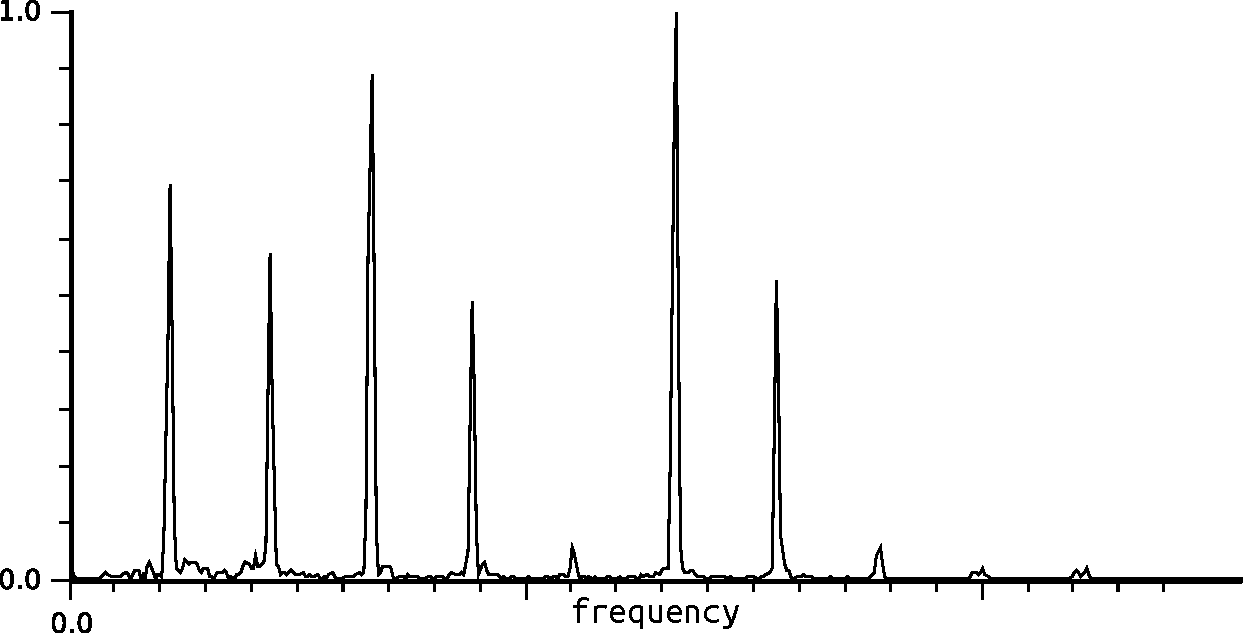
\includegraphics[width=0.90\linewidth]{test_image-1.pdf}
\caption{Spectrogram of a piano note A3 in vector graphics (PDF).}
\label{fig:example_1}
\end{figure}

For line drawings, vector graphics file formats like EPS or PDF are preferred
when available. When including figures in raster graphics file formats like
JPG or PNG, please try to generate an image of the appropriate size and
quality. (See Fig.~\ref{fig:example_2})

Figures should be numbered and should have a caption which should always be
positioned \emph{under} the figures, in contrast to the caption belonging
to a table, which should always appear \emph{above} the table; this is
simply achieved as matter of sequence in your source.

\begin{figure}
\centering
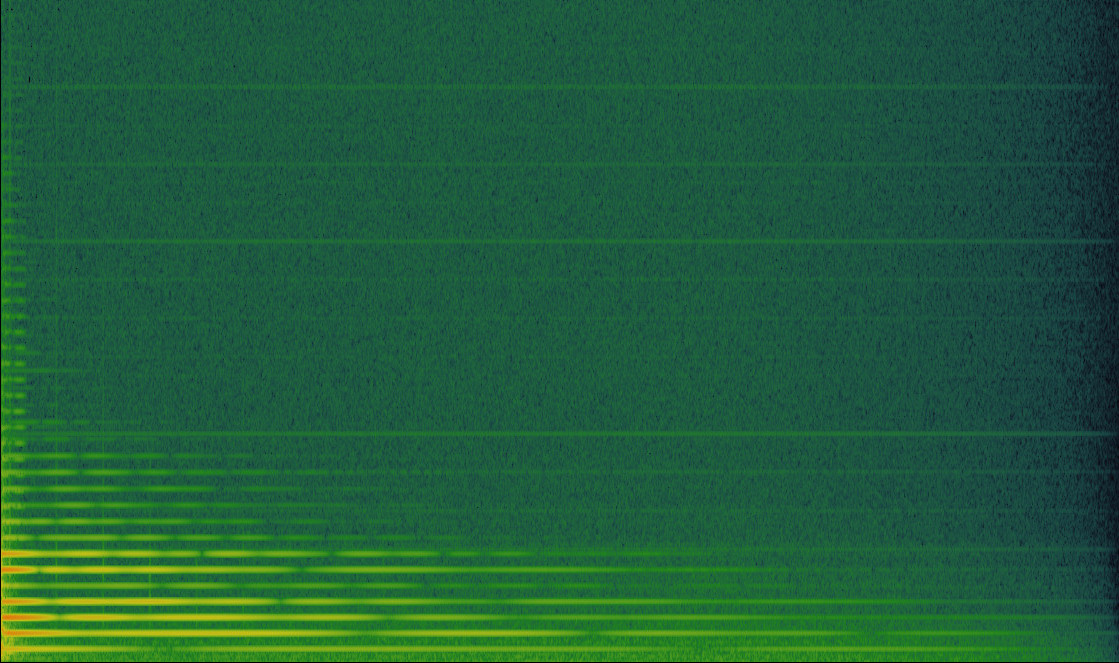
\includegraphics[width=0.90\linewidth]{test_image-2.pdf}
\caption{Spectrogram of the same sound file in raster image (JPG,
1119 x  663 pixels).}
\label{fig:example_2}
\end{figure}

Please define figures (and tables) as floating objects, and avoid using
optional location parameters like ``\verb+[h]+" for ``here".

\paragraph{Remark.}

The proceedings will be distributed only in electronic format, and colored
images are welcome. It would be convenient, however, to make sure that all
the images remain clear and legible when printed in black and white.

\subsection{Footnotes}

The superscript numeral used to refer to a footnote appears in the text
either directly after the word to be discussed or -- in relation to a
phrase or a sentence -- following the punctuation sign (comma, semicolon,
or period).\footnote{Example of a footnote.}

\subsection{Program Code}

Program listings or program commands in the text should use the \verb+verbatim+
environment: \\ \verb+csound -o dac foo.csd+.

\medskip

\noindent
{\it Example of Program Code}
	\begin{verbatim}
<CsoundSynthesizer>
<CsInstruments>

sr     =   48000
ksmps  =   8
0dbfs  =   1

instr  1

idur   =   p3
iamp   =   ampdbfs(p4)
ifreq  =   cpspch(p5)
kamp   linen  iamp, 0.1, idur, 0.3
a1     poscil kamp, ifreq
       out    a1

endin

</CsInstruments>
<CsScore>

i1 0   1   -3   8.00
i1 +   .   -6   8.01
i1 +   .   -4.5 8.07

</CsScore>
</CsoundSynthesizer>
	\end{verbatim}
%
\noindent
{\small Example Csound CSD file.}

\subsection{Citations}

For citations in the text please use square brackets and consecutive
numbers: \cite{jour}, \cite{proceeding} -- provided automatically
by \LaTeX 's \verb|\cite| \dots\verb|\bibitem| mechanism.

\subsection{Page Numbering and Running Heads}

Pages are numbered automatically. If the paper title is too long to serve
as a running head, it will be shortened. A shorter version of the title can
be provided with the \verb+\titlerunning+ command at the beginning of the
\verb+\document+ section.


\section{The References Section}\label{references}

Only references written using the Latin alphabet are accepted. If the title of
the reference uses a different alphabet, please use the transcript or
translation of the title, followed by the original language in parenthesis, e.
g. (in Russian) or (in Chinese).

The following section shows a sample reference list with entries for
journal articles \cite{jour}, books \cite{book1}, \cite{book2}, book chapter
\cite{chapter}, proceedings without editors \cite{proceeding}, as well as a
URL \cite{url}.

\begin{thebibliography}{4}

\bibitem{jour} Lorrain, D.: A panoply of stochastic `cannons'. Computer Music Journal 4(1), 53--81 (1980)

\bibitem{book1} Dodge, C., Jerse, C.: Computer Music: Synthesis, Composition and 
Performance, 2nd edn. Schirmer, New York (1997)

\bibitem{book2} Lazzarini, V. et al.: Csound: A Sound and Music Computing System.
Springer (2016)

\bibitem{chapter} ffitch, J.: Introduction to program design. In: R. Boulanger,
V. Lazzarini (eds.) The Audio Programming Book, pp. 383--430.
MIT Press, Cambridge (2010)

\bibitem{proceeding} Vercoe, B.: Real-Time Csound, Software Synthesis with
Sensing and Control. In: Proceedings of the International Computer Music
Conference, pp. 209--211. Glasgow (1990)

\bibitem{url} Csound Github site, \url{http://csound.github.io}


\end{thebibliography}



\end{document}
